\chapter{The Rules}
\setcounter{bestiarychapter}{\thechapter}

\section{Basic Actions}

\begin{multicols}{2}

\begin{wrapfigure}{R}{.2\textwidth}

	\begin{rollchart}

		{\bf \glsentrytext{tn}} & {\bf Task} \\\hline

		2 & Automatic \\

		4 & Trivial \\

		6 & Easy \\

		8 & Serious \\

		10 & Challenging \\

		12 & Heroic \\

		14 & Extreme \\

		16 & Epic \\

		18 & Legendary \\

		20 & Impossible \\

	\end{rollchart}

\end{wrapfigure}

\index{Simple Actions}
\noindent
A basic action is performed by rolling $2D6$ equal or higher than the \gls{tn} for the action.
The more difficult the action, the higher the \gls{tn}.
Players add their character's Attribute and Skill to the roll.
Attributes and Skills usually go as high as +3, so a +6 bonus is possible.
Very poor characters may be rolling with penalties if Attributes are sufficiently low.
\iftoggle{verbose}{All actions are assumed to have a \gls{tn} of 7 unless your \gls{gm} states otherwise.
Don't ask -- just roll!

\begin{exampletext}

When they arrived at the town of Arano they could already see the mountain their bard was supposedly wandering over in the distance. It was peaceful, but Arano was in complete disarray. People were nipping back and forth with cartloads of breads and smoked meats while others were rushing past with no discernible purpose.

Thenton needed information on whether or not that bard had travelled through here, how long ago and whether anyone noticed anything strange about his book, or singing. He had no desire to wait until things calmed down of their own accord - he would need to leave today.

Thenton's player uses his Intelligence Bonus (0) and Empathy Skill (+1).
The \gls{gm} stated no \gls{tn} so the \gls{tn} is 7.
Thenton's player rolls $2D6+1$ and the dice show a 4 and a 1, for a grand total of 6.
The roll is a failure.
No information about the bard is forthcoming, but the \gls{gm} still has some response to describe from the villagers.

After stopping several people they frantically explained that hobgoblins had attacked the last village before the South mountains - Casarenna.
The strange man-devouring monsters had been pushed back but the village would still be in need of military aid.
Apparently the mountains were full of hobgoblins, waiting to come down and eat everything.

Thenton suddenly regretted his views on that two hundred gold coin reward. He was almost certain his companions would turn back, but his dwarvish companion, Hugi, surprised him.

	\emph{Laddie, listen. Them dwarves in that there mountain hae a pact wi' a village o' yonder side o' the mountains. They telt them that if ever there was worry, they'd protect them. As a result the village hae always gi'en em aw're best meats fer cheap. An wan o' them just happens tae be ma cousin. A'm afraid Ah'm honour bound tae gang over the mountain and warn the village on the other side o' the coming storm, e`en if every last guid dwarf dwellin' thar be deed.}

Thenton thought for a moment. If Hugi was at all upset by all the other dwarves in the mountain being killed by hobgoblins, his cousin presumably included, he didn't show it.
Still, it was important to warn anyone who didn't know.
An unexpected hobgoblin attack could spread like wildfire before being put down, at least if people are not prepared.

Arneson nodded too.
The three were in agreement.
They would go across the mountains, capture their bard in the South Kingdom and then warn those people about the hobgoblins in the mountains.
But first Thenton would still have to get the villagers to tell him about the bard, and where he went.
\end{exampletext}
}{}

\subsection{\glsentrytext{restingaction}}\label{restingactions}

The basic system assumes that actions are taken while the player is being hurried.
When taking one's time is possible, things become much easier.
Exactly how much time is required is up to the \gls{gm}, but it can easily be several nights.
Sneaking into a house is a challenge, but much easier when one can take one's time, looking at it night after night to see if there is any breach in security.
Getting the latest gossip from a new village in a night is a normal action, but staying for a week and drinking every night with a different local is a \gls{restingaction}.

When taking a \gls{restingaction}, one die is presumed to have rolled a 6 and the player simply rolls the other die to obtain a result.

\iftoggle{verbose}{

\begin{exampletext}

	Thenton's player decides to retry his questions as a \gls{restingaction}.
	He already rolled the dice, so he cannot change the result by rerolling; the dice have decided that the village is far too frantic to help with random questions about long-forgotten strangers.
	Thenton's player instead takes the die that landed on a 1 and changes it to a 6.
	His total is now 8 and he has passed the test.
	This means the trio will have to spend longer than anticipated in the village and will not reach the other village until nightfall.

	After speaking with several villagers he found a single boy who remembered. \emph{These men came for him. They came and surrounded him and said they wanted his book, but then he just started singing, and they all went to sleep. After that he headed over to Caserenna. He must be trying to go over the mountain where the dwarves live. He had a funny accent and I think he came from the South, over those mountains}. Thenton suspected that the spell in the bard's book was some kind of sleeping spell. If he wasn't simply a very boring singer then the trio would have to strike fast if they found him, before he could send them all to sleep.

\end{exampletext}
}{}

\subsection{Teamwork}\label{teamwork}\index{Teamwork}\index{Group actions}

Some tasks lend themselves to working with others. Others can be difficult or impossible to do with companions. Some tasks, such as fleeing or sneaking, do not benefit at all from having a load of friends right behind you.

When acting as a group provides no benefit, one player rolls the dice and the same result counts for everyone.  If that player rolls a 9, then everyone's score is 9 and they add their own bonuses and penalties.

If, on the other hand, working together can benefit a situation, one character takes the lead, and up to three other characters can add up to half their bonus (rounded down).  Two companions with a +3 bonus would add a total of a +2 bonus.

\iftoggle{verbose}{

\begin{exampletext}

	Thenton wants to know what exactly that spell-song the boy was talking about means. He has the Academics Skill and never wrote down any specialisations so he asks the \gls{gm} if he can take a specialisation in whatever it is he needs in order to know about that bard and what he was up to. The \gls{gm} tells him to write down `Music' -- it's a fitting specialisation since he already plays the flute.

	Thenton then needs to roll using his Intelligence Bonus and Academics Skill -- the first is at 0 but his Academics Skill grants him +1.
The more academics you have, the better the chances that one of them knows something, so Hugi's player wants to help using his +2 Bonus.
He has Intelligence +1 and the Academics Skill at first level.
He wants to use his specialisation in History, and the \gls{gm} allows it.
Hugi is helping the action so he can add half his score of +3 (rounded down) for an additional +1 bonus.
Arneson has no knowledge of academic matters and an Intelligence Attribute at -1 so he's better off staying quiet.
Adding the bonuses together, the roll is at +2.
The \gls{gm} stipulates the \gls{tn} of 14 -- a tall order without a library to aid matters.
The roll fails and the troop will have to go into the situation blind.

Thenton recalled what the old alchemist had said about the book -- surely the bard had sung the song from the stolen book and put the guards to sleep with this magic. He searched his mind for where such a song might come from and what else it might be capable of. He wondered if the bard had really come from the South and what he might want with that book. The entire thing was an impenetrable enigma.

\end{exampletext}
}{}

\subsection{Resisted Actions}\index{Resisted Actions}

When \glspl{pc} come into disagreements with \glspl{npc}, the \glspl{pc} pick up the dice, and roll.  The \gls{npc}'s Traits add to the \gls{tn}.

For example, if a player attempts to pick someone's pocket, the \gls{npc} never rolls Wits + Vigilance.
Instead, if an \gls{npc} has a Wits + Vigilance total of +4, the \gls{tn} for the roll is $7 + 4 = 11$.
The player then rolls against that \gls{tn}.
The results are exactly the same, but having Players roll for everything helps emphasize agency and can speed up the game.

\iftoggle{verbose}{

\begin{exampletext}

	Arneson, Thenton and Hugi left that day, and as the sun was setting they saw Casarenna's smoking chimneys ahead, reaching up to the imposing, grey mountains behind. The smell of roasted meat was coming from every house.

	Unknown to the characters, the hobgoblins returned to attack the village again some hours ago, slaughtered everyone and began to roast them.
Hobgoblins tend to act quickly.
The smell of roasted meat is coming from human flesh roasting over each fire in the village, while little troves of hobgoblins each sit around one hearth, hungrily gnawing on undercooked dinners.

	The \gls{gm} wants to know if the characters will notice the village is full of hobgoblins before hollering a greeting.
	They might manage to luck into stealthing through the environment, or might be caught unaware.
	She decides the appropriate roll is Wits + Stealth, and that the character with the lowest score should complete the task, since if any one of them give away their position it will spell bad news for each of them.

	The \gls{gm} thinks about the difficulty.
	On the one hand, it is dark (which makes hiding easier) and there are some signs of battle in the village, such as blood on the grass.
	On the other hand, the darkness stops the characters seeing the signs of battle.
	She decides that the various factors cancel each other out and keeps the base \gls{tn} of 7.
	She adds the hobgoblins' score to this - the highest score counts since any of of the hobgoblins might spot the characters, but all the hobgoblins have the same score.
	They have Wits -1 and no Vigilance Skill; the hobgoblins' score is added to the \gls{tn} for a final \gls{tn} of 6.
	Meanwhile, Thenton still has a Wits + Vigilance total of -1.

	Thenton's player rolls a total of 4.

	Thenton shouted out, `Hey there! We are here from \dots' but Hugi quickly jumps up to cover his mouth, saying

	``Nay, laddie! Can ye no smell wha's cookin'? Can ye no see the blood on the grass? This place is deed. Them buggers musta returned, and they're cooking the humans. We best be quiet''.

	Movement from the nearby cottages soon showed them it was too late. A full village of the enemy were here, and they were starting to react and shout warnings and orders to each other.

\end{exampletext}
}{}

\subsection{Margins}\index{Margins}

Most actions are either a success or a failure, but sometimes the \gls{gm} will request to know a roll's Margin -- i.e. just how well the character has succeeded at the task. The Margin is the number of points over the \gls{tn} a roll has gathered. If the \gls{tn} is 9 and a player scores 11 then the Margin is 2.

The \gls{gm} might use a Margin for some variable, for example a bard attempting to charm a crowd into giving him money might gain $2D6$ copper pieces plus the Margin, so if the Margin is 3 then he would get $2D6+3$ copper pieces.
Margins might also be used to gain bonuses on later rolls.
Someone attempting to impress a noble court might roll Charisma with the Tactics Skill; the bigger the Margin the more troops they will be trusted with.

\iftoggle{verbose}{

\begin{exampletext}

	While previously the players rolled to hide against their opponent's ability to spot them, this time they roll to see if they spot a hidden opponent. The character with the highest score is Arneson, with Wits 0 and Vigilance +1. The \gls{gm} decides that the hobgoblin should use his Speed Bonus of +1, and his Stealth Skill adds +1 again. The hobgoblins' score of +2 adds to the basic \gls{tn} of 7, producing a final \gls{tn} of 9. Arneson's player rolls $2D6$ to produce a final score of `12' - the roll is a success and the margin is 3. Since the margin is quite good, the \gls{gm} decides that the troop leave the area before they are engaged and gain a +3 bonus to running away.

	The thatched roof on the nearby cottage rustled and Arneson instinctively drew his companions back. They turned and ran before their adversary could make his leap down to meet them with his axe. They ran as swiftly as they could into the safety of the darkness surrounding Casarenna but the hobgoblins stampeded fast behind them, running as swiftly as they could with guttural cries and war songs which Thenton could only guess translated to something about dinner.

	\begin{wrapfigure}{r}{.3\textwidth}

		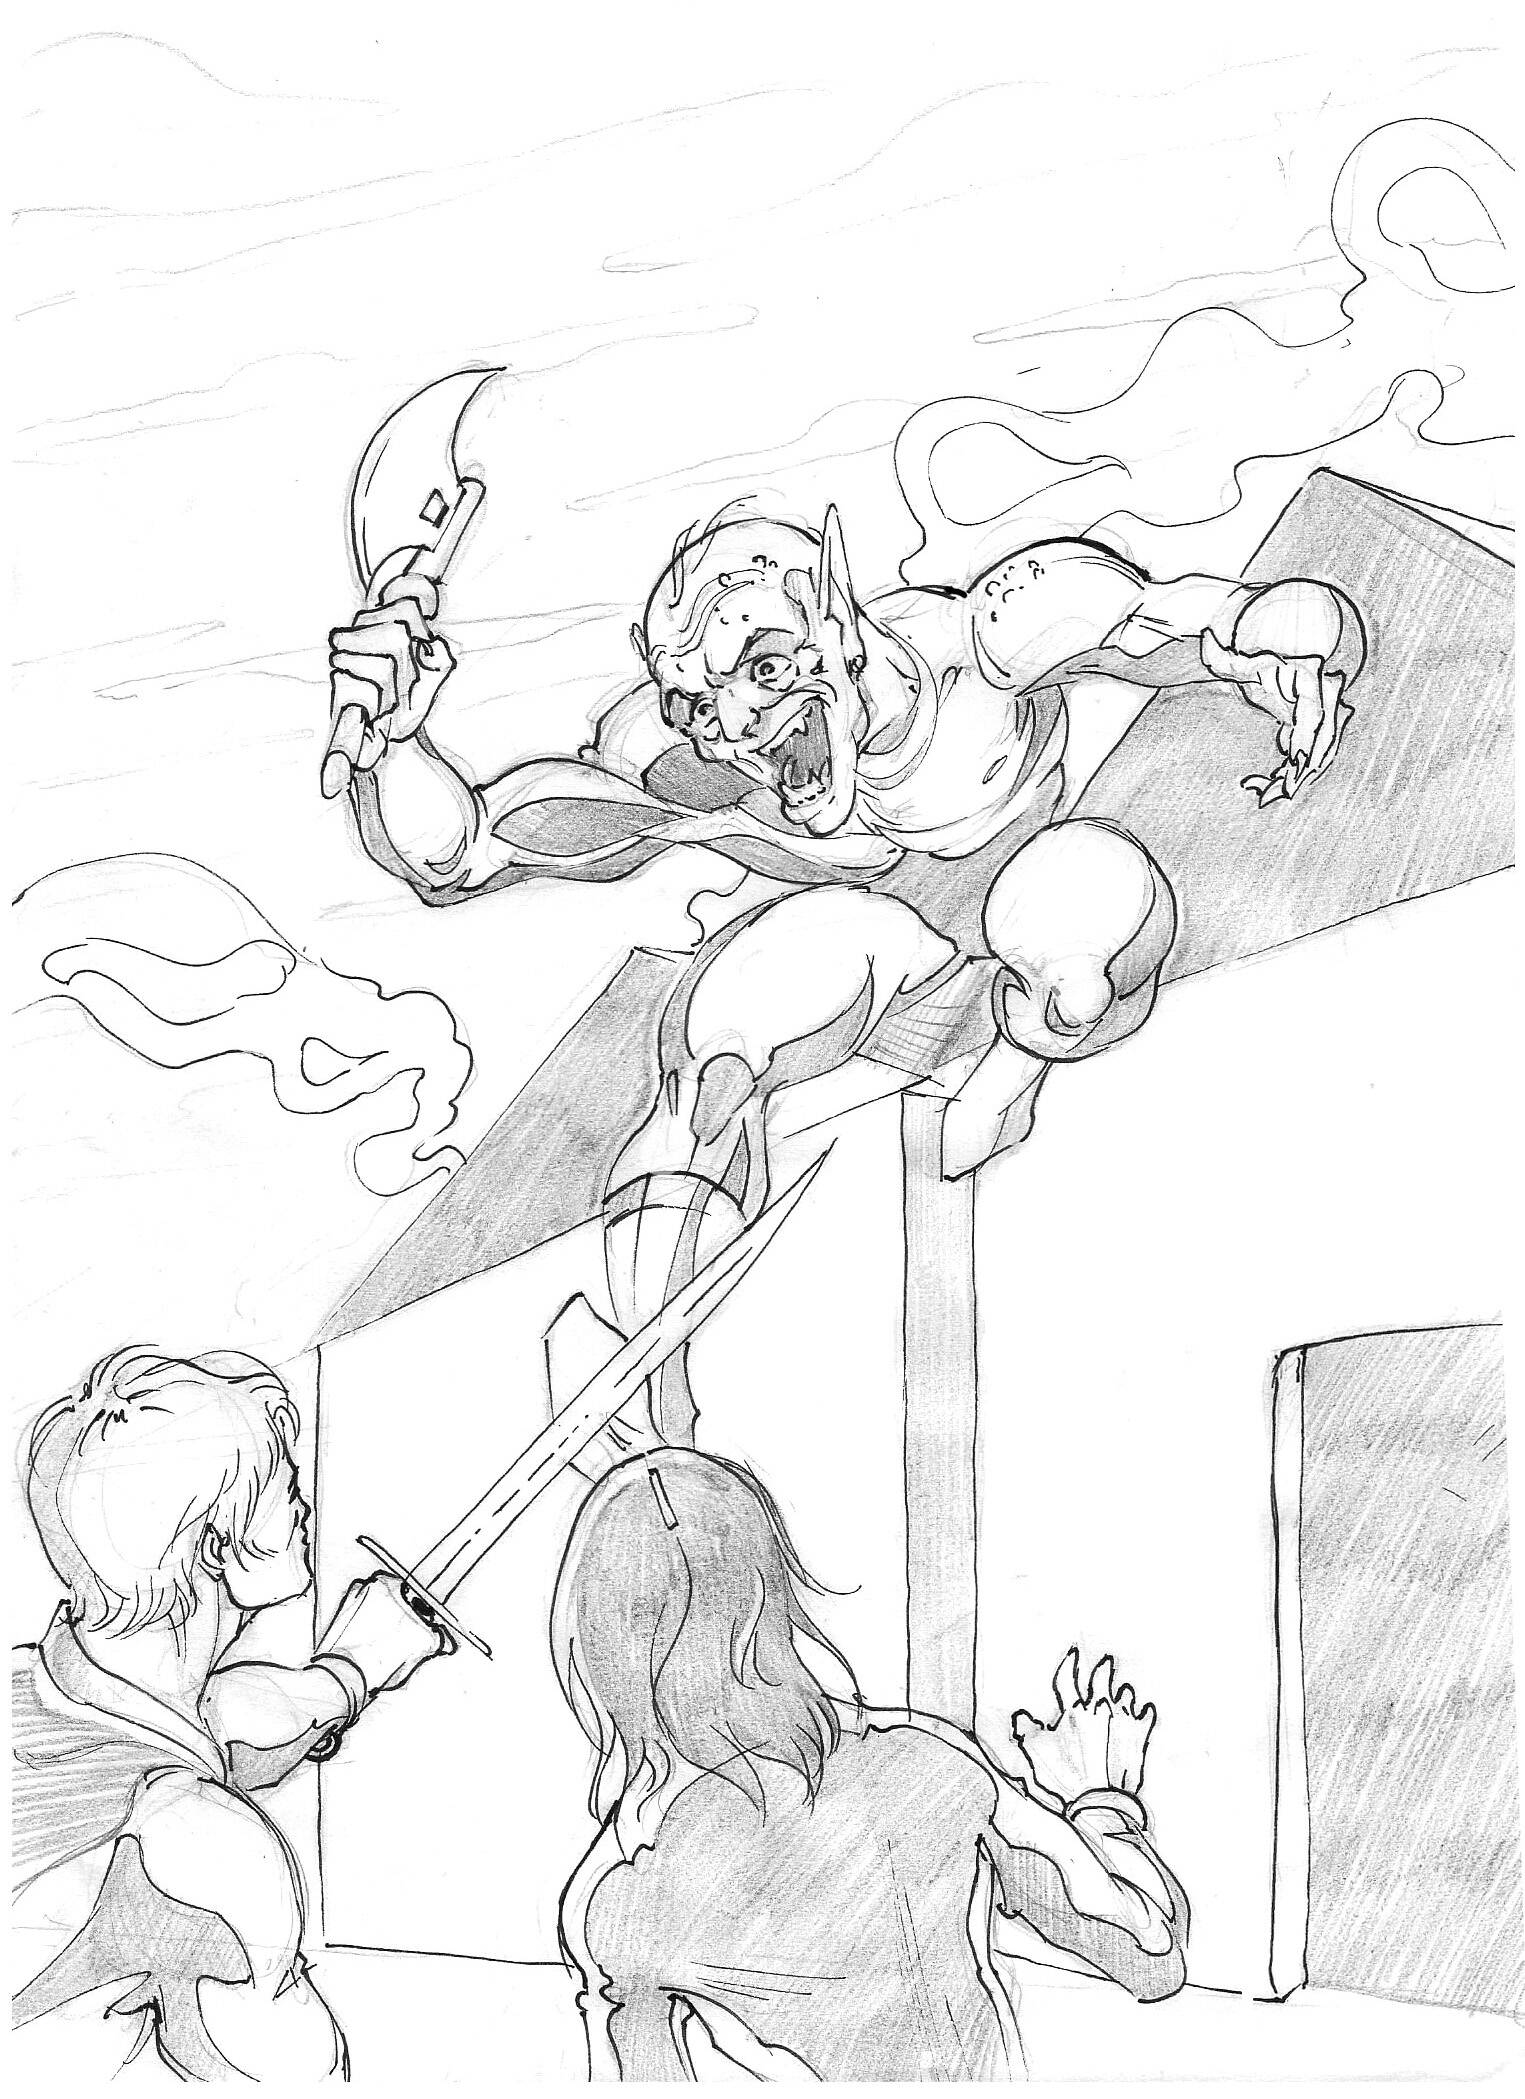
\includegraphics[width=\linewidth]{images/Boris_Pecikozic/nura_jump.jpg}
		\label{boris:jump}

	\end{wrapfigure}

	A scurrying of agile, hungry feet filled the little muddy rows between houses. The trio looked about for an escape route. Unknown to them, one of the hobgoblins was meant to be keeping a lookout from the roof of the cottage on the edge of town. He observed them for a brief moment and then jumped off, axe in hand, ready to make up for all the meals he had missed while pretending to keep guard.
	It was twenty long minutes of running before they were confident they were safe. Hugi and Thenton tenderly tried to regain their own breath while Arneson went to gather wood for a temporary shelter. Despite their distance from the village, they were kept awake by the wind bringing faint yet deep and reverberating songs from the village over to them all through the night.

	\end{exampletext}
}{}

\iftoggle{verbose}{
\subsection{What the Dice Mean}

You might think of the dice as representing random chance in the environment. Just how irritated is that person you're trying to question, and how creative is that craftsman feeling today? Dice are never re-rolled for different results on the same action because once the dice have told you what the situation is, the situation stays put.

}{
\subsection{No Rerolls}
Characters attempting to change a Standard Action into a \gls{restingaction} do not reroll but rather keep the same roll and turn one die up to show a 6, because while spending more time on a task can be very useful, sometimes the environment simply tells you `no'.
}%
Such a do-over still suggests initial failure; it just means that the character is trying over and over again until a better result is obtained.
Actions cannot be attempted multiple times with rerolls unless the situation has changed notably.

\end{multicols}

\section{Experience}
\label{xp}\index{Experience Points}

\begin{multicols}{2}

\noindent
As the story progresses, the \glspl{pc} gain \gls{xp}.
Each part of the character can be improved by spending \gls{xp}.
Buying basic stats is cheap while higher level stats quickly become extremely expensive.

\subsection{Gaining \gls{xp}}

Players receive \gls{xp} from the \gls{gm} for killing monsters, pious endeavours or fulfilling one's personal goals.
Larger and more dangerous monsters garner more \gls{xp}, as do grander missions.
\iftoggle{verbose}{The personal goals and piety of a character are denoted by different codes of belief and gods.
See page \pageref{gods_codes} for details on the gods and personal codes of honour.

\subsubsection{Training Time}

The \gls{gm} may wish to only award \gls{xp} at the end of a session, and may restrict when it can be spent.
Each Trait should increase by no more than a single level during the course of an adventure -- you might be lucky enough to get enough \gls{xp} to raise your Strength from -2 to +1 in a single session, but nobody can accrue that kind of muscle mass in such a short period of time.
Specialisation Skills such as Craft and Combat are difficult to train with, so it's recommended they only be bought during \gls{downtime}.
}

\subsubsection{What Counts?}

Enemies don't have to be killed for the \gls{xp}, merely `defeated'.
Any enemies fleeing count for half their \gls{xp} value so long as they engaged in one round of combat.

\subsection{Experience Points \& the Discount}

\iftoggle{verbose}{

Standing alone against a towering ogre is a nightmare, but three warriors standing against three ogres can be much easier.
A battle against thirty goblins can really take its toll, but three different battles against ten goblins can be child's play.
To represent this, we have \textit{the \gls{xp} Discount} -- a price you pay for every member of the party.

}{}

For every member of the party, that many points are deducted from one monster's \gls{xp} value (to a minimum of 0).
If the party has two members, the first two monsters have 2 \gls{xp} deducted from their total value.
If the party has five members, the first five monsters have 5 \gls{xp} deducted from their total.

\iftoggle{verbose}{

If a single warrior defeats a dragon worth 22 \gls{xp}, then the warrior receives 21 \gls{xp}, because 1 \gls{xp} is removed from the total.
If he fights 10 ghouls worth 2 \gls{xp} each, then he receives 1 for the first, and 2 for the rest, for a total of 19 \gls{xp}.

However, if five characters are fighting the 10 ghouls together, they each deduct 5 \gls{xp} from a single monster.
The first five ghouls are worth nothing, because each net ($2 - 5 = $) 0 \gls{xp}.
Only the last 5 ghouls count, bringing 10 \gls{xp} in total.  Dividing this among 5 players, each receives 2 \gls{xp} at the end.

}{}

If players need to discount multiple adversaries, they are counted from highest to lowest \gls{xp} value.

\subsection{Spending \gls{xp}}

Each additional level of a Trait has a steeply progressive cost. The costs represent buying the next level; the first level of a school of magic costs 15 and the second costs 20 -- buying up to the second level costs 35 \gls{xp} in total. Knacks work similarly, where the first Knack costs only 5 \gls{xp}, but the second Knack a Player purchases costs 10, and so on, with each additional Knack costing an additional 5 \gls{xp}.

\iftoggle{verbose}{

	\begin{wrapfigure}[13]{l}{.6\linewidth}

		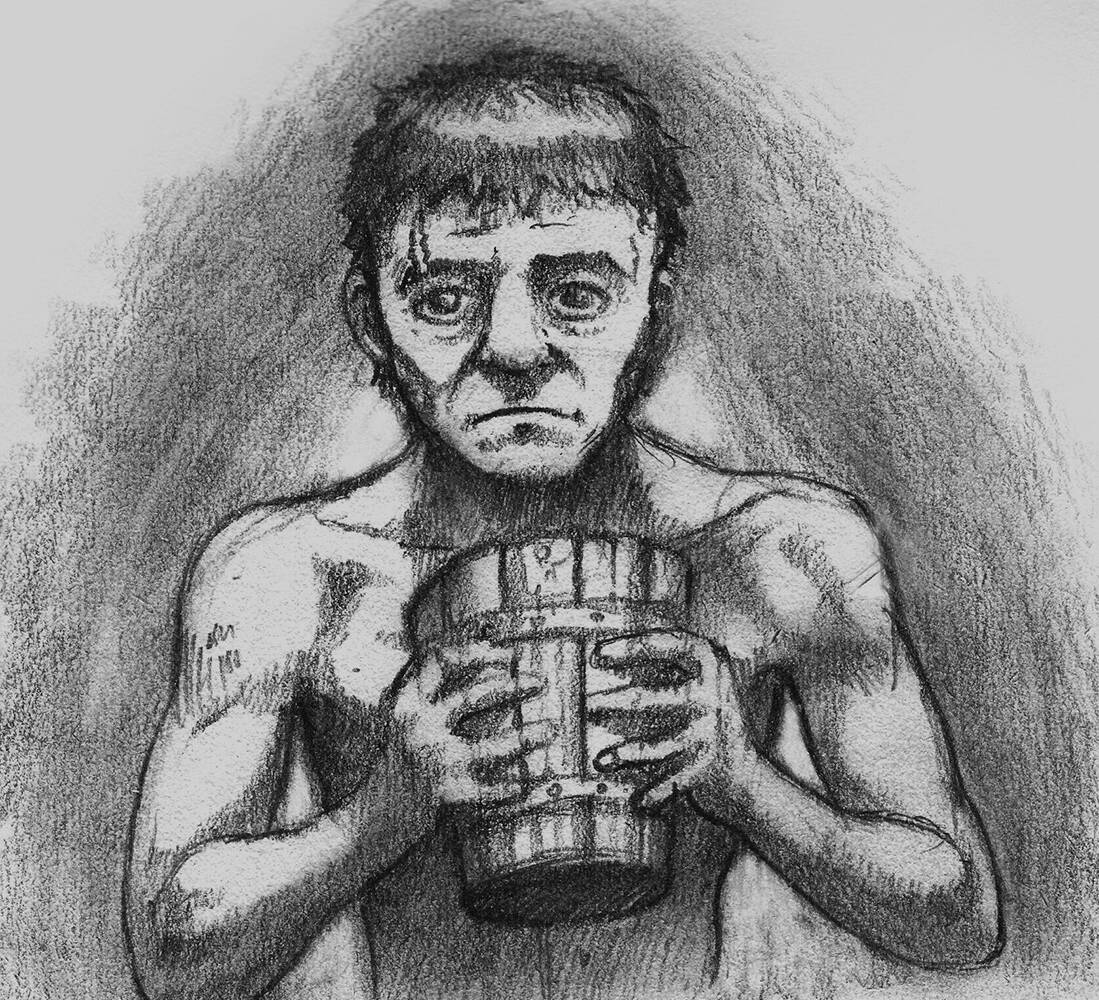
\includegraphics[width=\linewidth]{images/Roch_Hercka/xp-1.jpg}
		\label{roch:xp1}	

	\end{wrapfigure}

}{}

Attributes have a standard maximum of +3 and minimum of -3. This is adjusted by race, so for instance elves have a +1 bonus to Wits but -1 to Strength, so their maximum Strength score would be 2 and the minimum -4, while the maximum Wits is +4 and the minimum -2.

Buying off a negative level increases it by 1 and always costs 5 \gls{xp}, so taking a character from -4 Strength to 0 would cost 20 \gls{xp}.

		\setcounter{xp}{10}
		\newcounter{bon}\setcounter{bon}{1}

\begin{multicols}{2}

\begin{xpbox}{A}
		Attribute Level & Cost \\\hline

		Buy off negative & 5 \\

		+\arabic{bon} & \arabic{xp} \addtocounter{xp}{\value{bon}}\addtocounter{bon}{1} \\ 

		+2 & 20 \\

		+3 & 30 \\

		+4 & 50 \\
\end{xpbox}

\begin{xpbox}{A}

		FP Base & Cost \\\hline

		10 & 10 \\

		15 & 15 \\

		20 & 25 \\

		25 & 45 \\

		30 & 85 \\

\end{xpbox} 

\end{multicols}

\begin{multicols}{2}

\begin{xpbox}{B}

		Mana Base & Cost \\\hline

		2 & 5 \\

		4 & 10 \\

		6 & 20 \\

		8 & 40 \\

		10 & 80

\end{xpbox}

\begin{xpbox}{B}

		Magic Sphere & Cost \\\hline

		1st & 10 \\

		2nd & 15 \\

		3rd & 25 \\

		4th & 45 \\

		5th & 85

\end{xpbox}

\end{multicols}

\begin{multicols}{2}

\begin{xpbox}{C}

		Skill Level & Cost \\\hline

		+1 & 5 \\

		+2 & 10 \\

		+3 & 15 \\

\end{xpbox}

\begin{xpbox}{C}

		Combat/Proj. & Cost \\\hline

		+1 & 10 \\

		+2 & 20 \\

		+3 & 40 \\

\end{xpbox}

\end{multicols}

\iftoggle{verbose}{

\subsection{Concept}

Now is the time to look at your character's base Attributes and think about what they might be good at. The best place to start is your highest Attribute. If you have a positive (or simply not negative) Intelligence score, making a spell caster is a good option. Buy off any Wits penalties and put a magic sphere down on the character sheet and a couple of \glsentrylongpl{mp}. Alternatively, if your highest Trait so far is a Body Attribute perhaps this character is more suited to being a fighter. Don't worry if you have negative Body Attributes -- your starting \gls{xp} can buy all of that up to 0 quite easily.

\begin{wrapfigure}{R}{.6\linewidth}

	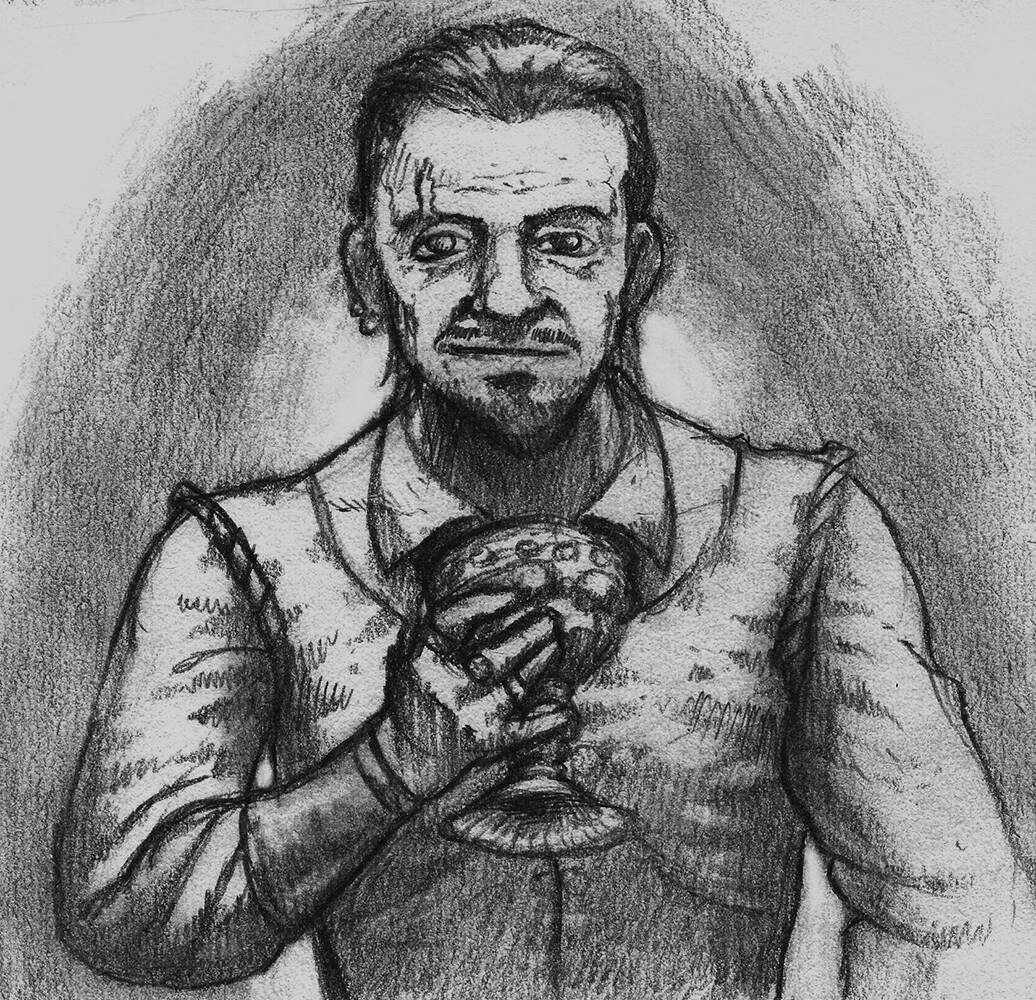
\includegraphics[width=\linewidth]{images/Roch_Hercka/xp-2.jpg}
	\label{roch:xp2}

\end{wrapfigure}

Mixed characters are easy to make -- a spell-casting, sword-swinging elf or a dwarf who prays to dark gods and sneaks well through the shadows simply requires a couple of Traits.
Think about which way the character is headed and at this point write something down in the character's `Concept' section at the top.
It might be something solid and classic, such as `sellsword', `eager paladin', `barbarian poet', `wizzard', or `greedy rogue'.
You could also wander off the traditional RPG model, playing a `lost outlander', `unwilling prophet' or `dishonoured noble'.

\begin{boxtext}

My own character, Thenton, has a good Charisma score and some basic ability to fight with his enhanced human Strength Attribute.
I think I'm going to make him a `knightly poet'.

\end{boxtext}

}{}

\subsubsection{Starting \gls{xp}}

Characters begin play with an amount of \gls{xp} stipulated by the \gls{gm} depending upon the level of their campaign.
The suggested starting \gls{xp} is 50, with up to 150 \gls{xp} for more advanced campaigns.
\iftoggle{verbose}{With that in mind, it's time for me to spend some of that 50 \gls{xp} on Thenton, the knightly poet.

For a start, he'll need the Performance Skill, and he gets two specialisations with it because it's a specialised Skill.
`Poetry' is a good start, and perhaps the flute after that, because why not? That costs 5 \gls{xp} so I have 45 left.
He should have some basic Combat ability, so I'm going to give him +1 in the Combat Skill -- that'll cost 10, and why not put him at +2 for another 20 \gls{xp}? That leaves only 15 \gls{xp} to go.
Since he's a fighter he needs the Dexterity penalty removed.
Removing the penalty costs only 5 \gls{xp}, so with 10 left I'm going to buy a level of Empathy to make him a socialite.
Deceit would also be good, but I think a knightly poet would be too naive for that.
Finally, a member of the nobility, even a minor noble, should have some basic Academics knowledge, so his last Trait will be the first level of the Academics Skill.
}{}

\end{multicols}

\section{Gold \& Goods}\label{goods}\index{Equipment}

\begin{multicols}{2}

\subsection{Money}\index{Money}

An open ended list of equipment is provided to give a basic idea of costs.
The basic coinage covered here is human coinage, but each culture will use their own currency and exchange rates.
A hundred \glsentryfullpl{cp} is worth 1 \glsentryfull{sp}.
10 \glspl{sp} is worth 1 \glsentryfull{gp}.

An average villager will make little spare money -- perhaps 10 \glspl{sp} in a year if they bother to save.
Sellswords can expect to make upwards to 10 gold per year if they are hired by a villagemaster.
The average free trader -- a blacksmith or cloth dyer -- can expect to make 5 \gls{sp} in a month.

Prices for weapons are placed next to the weapon in chapter \ref{combat}, page \pageref{weaponschart}.

\begin{tcolorbox}[arc=1mm,tabularx={p{.3\textwidth}XX}]

	\textbf{Animal} & & \textbf{Cost} \\\hline

	Dog & & 2 sp \\

	Donkey &   &  2 sp \\

	Horse &   &  5 gp \\

	War Horse &   &  8 gp \\

	Leather Barding &   &  10 sp \\

	Chain Barding &   &  20 sp \\

	Plate Barding &   &  18 sp \\\hline

\end{tcolorbox}

\begin{tcolorbox}[arc=1mm,tabularx={p{.3\textwidth}XX}]

	\textbf{Buildings} & & \textbf{Cost} \\\hline

	Cottage & &  20 gp \\

	Keep & &  1,000 gp \\

	Small Castle & &  4,000 gp \\

	Medium Castle & &  10,000 gp \\

	Large Castle & &  30,000 gp \\\hline

\end{tcolorbox}

\begin{tcolorbox}[arc=1mm,tabularx={p{.3\textwidth}XX}]

	\textbf{Clothing} & \textbf{Weight} & \textbf{Cost} \\\hline

	Peasant clothes &  -3 &  50 cp \\

	Noble clothes &  -4 &  1 gp \\

	Lavish clothes &  -5 &  3 gp \\

	Travelling clothes &  -3 &  5 sp \\

\end{tcolorbox}

\begin{tcolorbox}[arc=1mm,tabularx={p{.3\textwidth}XX}]

	\textbf{Professional Tools} & \textbf{Weight} & \textbf{Cost} \\\hline

	Cart & 11 & 10 gp \\

	Grappling hook &  -2 &  1 sp \\

	Ink bottle &  &  5 cp \\

	Iron rations &  -2 &  10 cp \\

	Lantern &  -2 &  3 sp \\

	Lock pick set &   &  10 sp \\

	Metallurgy set &  6 &  40 sp \\

	Parchment sheet &   &  1 cp \\

	Quill &   &  4 cp \\

	Rope, 50' &  -1 &  50 cp \\

	Rope, silk, 50' &  -4 &  3 sp \\\hline

\end{tcolorbox}

\index{Camping}
\begin{tcolorbox}[arc=1mm,tabularx={XX}]

	\textbf{Travel} & \textbf{Cost} \\\hline

	Ale &  1 cp \\

	Cart &  1 gp \\

	Camping equipment & {1 sp} \\

	One meal & 2 cp \\

	One meal & 2 cp \\

	Barn for the night & 2 cp \\

	Basic room for the night & 30 cp \\

	Fancy room for the night & 3 sp \\\hline

\end{tcolorbox}

\subsection{Working Beasts}

Animal stats vary, but you can use the below as a go-to standard for working animals.
Quadrupeds can run at double the standard speed when going full pace, so horses can allow a party to travel at far higher speeds than normal.

\settoggle{examplecharacter}{true}
\horse

\settoggle{examplecharacter}{true}
\warhorse

\settoggle{examplecharacter}{true}
\huntingdog[\npc{\A}{Hunting Dog}]

\subsection{Weight \& Encumbrance}\index{Weight}\index{Encumbrance}

We measure weight in broad terms.  Characters have a \textit{weightrating} equal to their \gls{hp}, so elves tend to have 5, while humans tend to have a \gls{weightrating} of 7.
Items work similarly, with \gls{weightrating} between -4 (for very light items) and +11 (for wardrobes, carts, and boulders).

\iftoggle{verbose}{
	\noindent\includegraphics[width=\linewidth]{images/Roch_Hercka/dwarf_encumbrance.jpg}
	\label{roch:dwarf}
}{} 

If an item's \gls{weightrating} is equal or below your character's Strength, you can lift it easily.
However, if the items has a greater \gls{weightrating} than your Strength Bonus, you gain a point of Encumbrance for every increment that item is above your Strength Bonus.
Encumbrance slows you down and makes you tired, detracting from your Speed Bonus, and adding to your Fatigue each Scene.

Characters can carry items with a maximum \gls{weightrating} of their Strength Bonus plus 6, so a man with 7 \gls{hp} could only be carried with a Strength Bonus of +1 or greater.  Depending upon the circumstances, the \gls{gm} may allow heavier objects to be dragged or rolled.

Items carried in only one hand count as having +2 to the \gls{weightrating}, so hefting a battle axe in only one hand would mean it has an effective \gls{weightrating} of 5.

Characters cannot carry any item which gives them a -5 Encumbrance rating or higher.

\iftoggle{verbose}{

\begin{exampletext}

	For example, Thenton, with a Strength Bonus of +1, picks up a weighty battle axe. The \gls{weightrating} is 3, so this inflicts an Encumbrance Penalty of 2.
Thenton's effective Speed Bonus drops to -2, reducing his Initiative (covered below) and ability to run.
He will also gain 2 Fatigue points at the end of each scene\footnote{See page \pageref{time} for notes on scenes.} where he carries it.

\end{exampletext}

}{}

\subsection{Services}

Money can buy you more than things.  In fact, for the right money in a large city, characters can buy a full entourage.  Villages, however, will not admit of the same opportunities.

The costs below show the starting price for a few services, plus additional fees for the details.
For example, hiring a guide for an uncharted and dangerous area for 5 days would cost 800 \glspl{cp}.

\end{multicols}

\begin{tcolorbox}[arc=1mm,tabularx={XX},title=Services]

	\textbf{Sellsword} & 10sp/ day \\\hline

	Opponent & \gls{xp}$^3$ sp \\

	Illegal Murder & 10sp \\\hline

	\textbf{Guide} &  150 cp/ day \\\hline

	Dangerous area & 1sp \\

	Uncharted area & 50cp \\\hline

	\textbf{Minstrel} &  15 cp/ performance \\\hline

	Large audience & 500cp \\

	Massive audience & 1sp \\

	Creating a new song & 2sp \\

	Illegal song & 5sp \\\hline

	\textbf{Tracker} &  5 sp/ day \\\hline

	Dangerous area & 2sp \\

	Uncharted area & 4sp \\

\end{tcolorbox}

\begin{multicols}{2}

\subsection{Cultures \& Exchange Rates}

\index{Exchange Rates}Different cultures have different exchange rates -- the elven versions of standard equipment are always artistically engraved and in high demand; the elves also value the coinage and materials of outsiders very little, so they will not part with their items for human or dwarvish gold easily. As a result, their -- and other -- culture's items are more expensive than human items. The costs of the items here are based on the most common race -- humans. Other races have a multiplier effect based on how expensive their equipment is.

\needspace{6em}
\begin{wrapfigure}[9]{r}{.48\linewidth}

	\begin{rollchart}

		Race & Multiplier \\\hline

		Elves & $\times 3$ \\

		Dwarves & $\times 2$ \\

		Gnomes & $\times 2$ \\

		Gnolls & $\frac{1}{2}$ \\
		
		\vspace{.1cm} & \\

	\end{rollchart}

\end{wrapfigure}

Different races will also have different items available.
In general, anything of a basic (non adjusted) value of over 2 \gls{sp} will not be available in a village, while towns will not have anything of over 1 gp in value.
Characters can only buy expensive, artisan, items in cities.

\subsubsection{Starting Equipment}\label{start_equipment}

\index{Starting Equipment}
\index{Adventuring Equipment}
Characters begin with money, items, and \gls{adventuringequipment}.
Characters each start with one items per Skill level, and each item can be worth 10 \glspl{sp} or less.
This might include a sword, dagger, a donkey, or anything else worth 10 \gls{sp} or less.

The player can decide to replace any of these items with a generic item called \gls{adventuringequipment}.
If a player has an \gls{adventuringequipment} item, they can decided to describe exactly what it is at any point later in the game.

\begin{exampletext}

	Out in the forest, the group need some fire starting equipment.
	Luckily, Arneson's player put down three pieces of \gls{adventuringequipment}, which could be any number of things.
	He marks one off, and decides this particular piece of \gls{adventuringequipment} is a tinder box, so he can start a fire.

	Meanwhile, Hugi is out of rations, so his player marks his last piece of \gls{adventuringequipment} as a day's rations.

\end{exampletext}

\gls{adventuringequipment} can include any of the following items:

\begin{itemize}

\item{Chalk}
\item{Lock picking set}
\item{Medical equipment}
\item{Mirror}
\item{Rations for a day}
\item{Rope}
\item{Tinder box}
\item{Torch}
\item{Wine}
\item{Writing equipment}

\end{itemize}

\subsubsection{Starting Money}

The amount of bare money a character starts out with depends upon social class, which is indicated by their Skills.
Starting money is $3D6-5$\gls{cp}.
Multiply this result by 2 for every level in a specialist Skill the character has (meaning, those with an asterisk beside them).
Finally, characters with Academics times this result by 100 (effectively giving them \glspl{sp} instead of \glspl{cp}).

For example, a character with Academics 1 and Tactics 1 might roll a 7.
$7\times2\times2 = 28$, so the character starts out with 28\gls{sp}.

\iftoggle{verbose}{
	\begin{exampletext}

Thenton now only needs his starting equipment.
We covered already that he starts with any two items worth 10 \gls{sp} or less plus one more item per Skill.
The Combat Skill, Empathy and Performance let him start with 3 items in total.
We'll start with some shiny Partial chainmail and a longsword so he can fight.
His final item will be \gls{adventuringequipment}, so he'll have some flexibility for later.

Rolling $3D6$ for his starting money, I've got a `9', so I'm starting with 4 ($9-5=4$).
His three specialized skills double that number, making it 32 ($4\times2^3$).
Since one of those Skills is Academics, he'll start with 32 \glspl{sp} rather than \glspl{cp}.

	\end{exampletext}

\end{multicols}

\npc{\M}{Thenton}
\settoggle{examplecharacter}{true}

\person{1}{0}{0}{{0}{-1}{1}}{0}{2}{Academics 1, Empathy 1, Performance 1}{\longsword, \partialchain, \gls{adventuringequipment} x 1, 32\glspl{sp}}{}

}{

\end{multicols}

}

\section{Time \& Space}\label{space}\label{time}

\begin{multicols}{2}

\noindent
This game uses the entirely abstract measurements of the `scene' and `square' for time and space. They are more compliant to narrative than physics, and form the basis of all movement and actions whenever people start tracking how long something takes and where everyone is.

\subsection{Time as Scenes}

When everyone wants to talk and act at the same time, time is tracked in \glspl{round}.
This period of time is used almost exclusively while tracking combat.
The \gls{round} itself can then be further divided into Initiative Scores if you want real detail, but that's covered later.
All that matters is that a \gls{round} is a period of time in which people attempt to hit each other, then another \gls{round} occurs.

Most of the time, actions will not occur through \glspl{round} but rather scenes. A scene is just any unit of time in which the \glspl{pc} take on a task or two, usually within a single area. We track scenes only because a few game effects occur at the end of each scene -- mostly these are narrative effects such as regaining \glspl{fp}\footnote{See page \pageref{fate_points}.} in order to regain plot-immunity from Damage. The scene lasts until the \gls{gm} says that it's over.

Lastly, there is an adventure. The adventure lasts until the current plot-thread is resolved, or some period of `sandboxing' through a world until a proper use of one's time can be found.

\subsection{Space as Squares}\index{Space}\index{Squares}\index{Areas}

Space is tracked through \glspl{square}.
A \gls{square} is just any unit of space within the battlefield.
If you are using a battlemap which has squares marked out on it, then those squares are the size of a square, even if those squares happen to look very hexagonal.
A square might be ten metres wide as each one covers an entire house when the battlefield is a large town, or it might be just two yards wide when moving through a detailed map of a dungeon.
The precise distances represented do not matter, just so long as they consistently balance one character's ability to run away with another's ability to hit someone with a projectile.

The next unit of space is the `\gls{area}'.
An \gls{area} is just any \gls{area} which looks different from another.
While traipsing through a small dungeon, each room and cavern entered might be thought of as an \gls{area}.
When gallivanting through open plains one \gls{area} might be a copse of trees, another a lake, and then the next area a village.

The final unit is a `region'.
Regions encompasses a full forest, a town, or a collection of villages.
Each region has its own set of likely encounters, such as tradesmen in the villages, cut-throats in town, and elves in the forest.\footnote{If all this looks like a repugnant abstraction, just set a square to two yards, an area to one mile, a \gls{round} to six seconds and a scene to one hour.}

\end{multicols}


